% -- Approach ---------------------------------------
\section{Approach}
\label{sec:approach}
%Our extracted kernel can be found in appendix \ref{sec:satd}. 
The kernel can run in the $\rho$-VEX by putting the \mcode{bytecode} generated by the \mcode{makefile} into the instruction memory of the $\rho$-VEX and placing all required data in its data memory dynamically. By executing \mcode{make byte-} command two files are created:
\begin{itemize}
	\item \mcode{bytecode}, containing all the intstructions to be executed by the $\rho$-VEX
	\item \mcode{bytedata}, containing the pixels of the input stream
\end{itemize}

In order to make the extracted kernel qualified for compilation and execution, a few things have to be altered. First, the new file has to be recognized by the \mcode{makefile} in the rovex-examples directory. Second, some type definitions have to be made. Originally, \mcode{pixel\_satd\_8x4} resides in the \mcode{pixel.c} file of the x264 application. When extracting this kernel, all prior knowledge is lost and has to be defined again. Then, in order to make the kernel compile and run on the $\rho$-VEX, the development board has to be reset and started. \mcode{Bytecode} has to be written to the instruction memory (\mcode{rvex-imemory}) and \mcode{bytedata} to the data memory (\mcode{rvex-dmemory}). Finally, the calculated result should be returned to the host. Figure \ref{fig:rvex-dmem} shows the $\rho$-VEX memory layout for our kernel.
% --- dmem of the ROVEX ----------------------------------
\begin{figure}[htb]%
\centering
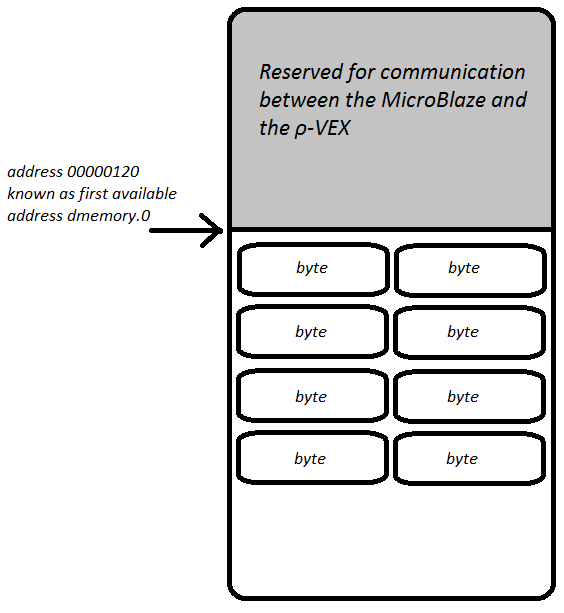
\includegraphics[height=200px]{Pictures/dmem_rvex}%
\caption{Memory layout of the $\rho$-VEX}%
\label{fig:rvex-dmem}%
\end{figure}

\subsection{Adjusting the \mcode{makefile}}
We added the kernel to the \mcode{EXECUTABLES} defined in the \mcode{makefile}. Other files defined here can be removed since we will not need them for our application. An important issue is the difference between logical memory and physical memory. While the first address of a logical memory is obviously address '0', the physical memory can have the first part of the register being occupied (e.g. by the operating system). For the $\rho$-VEX, the first address which is allowed to be written to is 0x120. Thus, when writing the result of the kernel to the logical address '0', it is  actually writing to the physical address '120' of the data memory. %This can be done using \mcode{\_\_DATA\_START} to indicate the start address.

Despite the fact that this is a rather simplistic operation, it took us some struggling to properly distinguish these address spaces. For example, we were told by the TA to remove the \mcode{autoinline} flag which resulted in a lot of wrong hexdumps. Also, the introduced fix discussed in \ref{sec:fix} caused some problems that took us until the end of the second week to resolve.

\subsection{Constraints of the $\rho$-VEX}
Using the $\rho$-VEX as a co-processor comes with some limitations. First, the $\rho$-VEX supports a very old and basic C compiler, so using \mcode{printf} statements to find bugs in the extracted kernel file is not possible. Everytime the application is being run concurrently on the $\rho$-VEX, the status is being inspected by placing \mcode{printf} statements in the \mcode{pixel.c} file, the origin of the kernel. Also, the $\rho$-VEX is very strict in the order of variable declarations and initialization. One of our bugs involved \mcode{int i} being declared and initialized, followed by a declaration of \mcode{int result}. This is not supported by the $\rho$-VEX, since it wants to have \mcode{int i, result;} both to be declared first, before initializing \mcode{i = 4;}.

When running an extracted kernel on the $\rho$-VEX, the kernel is unable to obtain information from previous code. Consequently, all parameters have to be re-defined. Table \ref{tab:typedef} shows all required type definitions.

% -- Type Definitions ---------------------------------------
\begin{table}[htb]%
\begin{tabular}{lll}
	\bf{Parameter} 					& \bf{Type definition} 					& \bf{Motivation}\\ \cline{1-3}
	\mcode{intptr\_t}				&	\mcode{unsigned int}					& This parameter represents the stride, which cannot be $<$0\\
	\mcode{pixel}						& \mcode{unsigned char}					&	Pixels are made out of bytes, which have 8 bits (like a \mcode{char})\\
	\mcode{sum\_t}					&	\mcode{short int}							& Same type definition as in the source code (16 bits)\\
	\mcode{sum2\_t}					& \mcode{long int}							& Same type definition as in the source code (32 bits)\\
	\mcode{BIT\_DEPTH}			& defined as 8									& Also in the source code, plus the kernel handles pixels (bytes)\\
	\mcode{BIT\_PER\_SUM}		&	(8 * \mcode{sizeof(sum\_t)})	& Also predefined as in the source code, being 16 \\
\end{tabular}
\caption{Type definitions in the extracted kernel file.}
\label{tab:typedef}
\end{table}


\subsection{Communication between the MicroBlaze and the $\rho$-VEX}

In order to delegate the \mcode{pixel\_satd\_8x4} kernel from the MicroBlaze to the $\rho$-VEX, both the environments need to communicate with each other. When executing the x264 application, the MicroBlaze has to load the instructions of the extracted kernel into the instruction memory of the $\rho$-VEX and the data (for which the SATD has to be evaluated) into the data memory. This is when the source code of x264 becomes involved. The \mcode{pixel\_satd\_8x4 kernel}, which is residing in the \mcode{pixel.c} file of the application, needs to be adjusted. Instead of calculating the SATD itself, it should send the instructions and input data to the $\rho$-VEX. The commands \mcode{open()}, \mcode{close()}, \mcode{read()} and \mcode{write()} are therefor added to the \mcode{pixel.c} file of the x264 application. These pixels are written at physical address 120, the first address on the $\rho$-VEX that is not set apart for communication between the driver and the $\rho$-VEX, defined as address '0'. To be sure that the data is always written to the same location we use the \mcode{lseek()} function to specify the start location of data as 0x00 from the \mcode{SEEK_SET}, or the beginning of the file. 

To control the $\rho$-VEX from the x264 application, the control registers can be written too. By writing \mcode{'2'} to the control registers, the $\rho$-VEX is being reset. It can then be started by writing \mcode{'1'} to the register, telling the $\rho$-VEX to start running the instructions available in the instruction memory, calculating the SATD of the two pixels. While calculating, the status of the $\rho$-VEX can be checked in a \mcode{while}-loop by reading the status variable of the status memory (\mcode{rvex-smemory}). When the kernel is finished, the result can be read from the data memory. See also \mcode{pixel.c}.

\subsection{Result Hyphothesis}

By having the computational intensive kernel being run concurrently on a co-processor, one would expect an overal speedup of the application. A problem is, however, that the \mcode{bytecode} and the data have to be sent to the $\rho$-VEX every time the kernel is being called. The data contains two new pixels of which the SATD has to be calculated, whereas \mcode{bytecode} holds the kernel instructions. Because of this constant data traffic between the MicroBlaze and the $\rho$-VEX we don't expect the intended speed up to be achieved.

The reason that \mcode{bytecode} has to be sent every time the kernel is called, is that the three available FPGAs are shared among a lot of students. When running their application concurrently, the instruction memory is constantly being overwritten by another group. If there was a one-to-one setup, \mcode{bytecode} could have to been placed in \mcode{main.c}, written tot the \mcode{imemory} of the $\rho$-VEX only once when starting the application. 


